\RequirePackage{ifluatex}

\ifluatex
  \RequirePackage{luatex85} % make it work with luatex
\fi

\documentclass[tikz]{standalone}

\usepackage{tikz, xcolor}

\usetikzlibrary{arrows.meta, calc} % arrow styles and calculation libraries

\newcommand{\dd}[2]{% double diffusion arrows
  \draw  [-Circle] ($(#1.north east)!0.7!(#1.north)$) -- ($(#2.south east)!0.7!(#2.south)$);
  \draw  [Circle-] ($(#1.north west)!0.7!(#1.north)$) -- ($(#2.south west)!0.7!(#2.south)$);
  }

\newcommand{\sd}[2]{% single diffusion arrows
  \draw [-Latex] (#1.east) -- (#2.west);
  }

\begin{document}
\nopagecolor
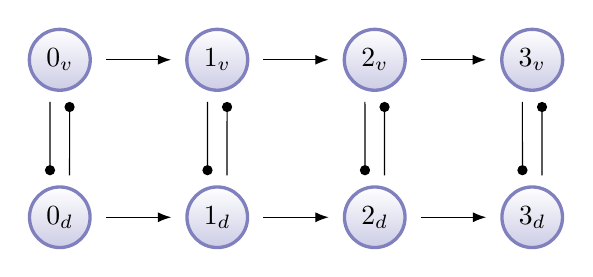
\begin{tikzpicture}[
  neuron/.style={
    % The shape:
    circle,
    % The size:
    minimum size=6mm,
    % The border:
    very thick,
    draw=blue!50!black!50,
        % The filling:
    top color=white,
    bottom color=blue!50!black!20, % and something else at the bottom
    % Font
    font=\itshape,
    % padding around node
    outer sep=2mm
  },
  ]

  % Loop to create neurons, integrates creation of 2 way coupling
  \foreach \i in {0, 1, 2, 3}
  {
    \node (\i d) [neuron] at ($(\i*2, 0)$) {$\i_d$};
    \node (\i v) [neuron] at ($(\i*2, 2)$) {$\i_v$};
    \dd{\i d}{\i v}
  }

  % loop for 1 way coupling
  \foreach \i/\j in {0/1, 1/2, 2/3}
  {
    \sd{\i d}{\j d}
    \sd{\i v}{\j v}
  }

  % draw `To additional neurons'
  % \draw [-Latex] (3v.east) -- ($(3v.east) + (1, 0)$) node [right] {Additional neurons};
  % \draw [-Latex] (3d.east) -- ($(3d.east) + (1, 0)$) node [right] {Additional neurons};

\end{tikzpicture}
\end{document}
